%-----------------------------------------
\begin{frame}
\frametitle{Tidal systems in operations}

\begin{minipage}{0.45\textwidth}
    \begin{figure}      
    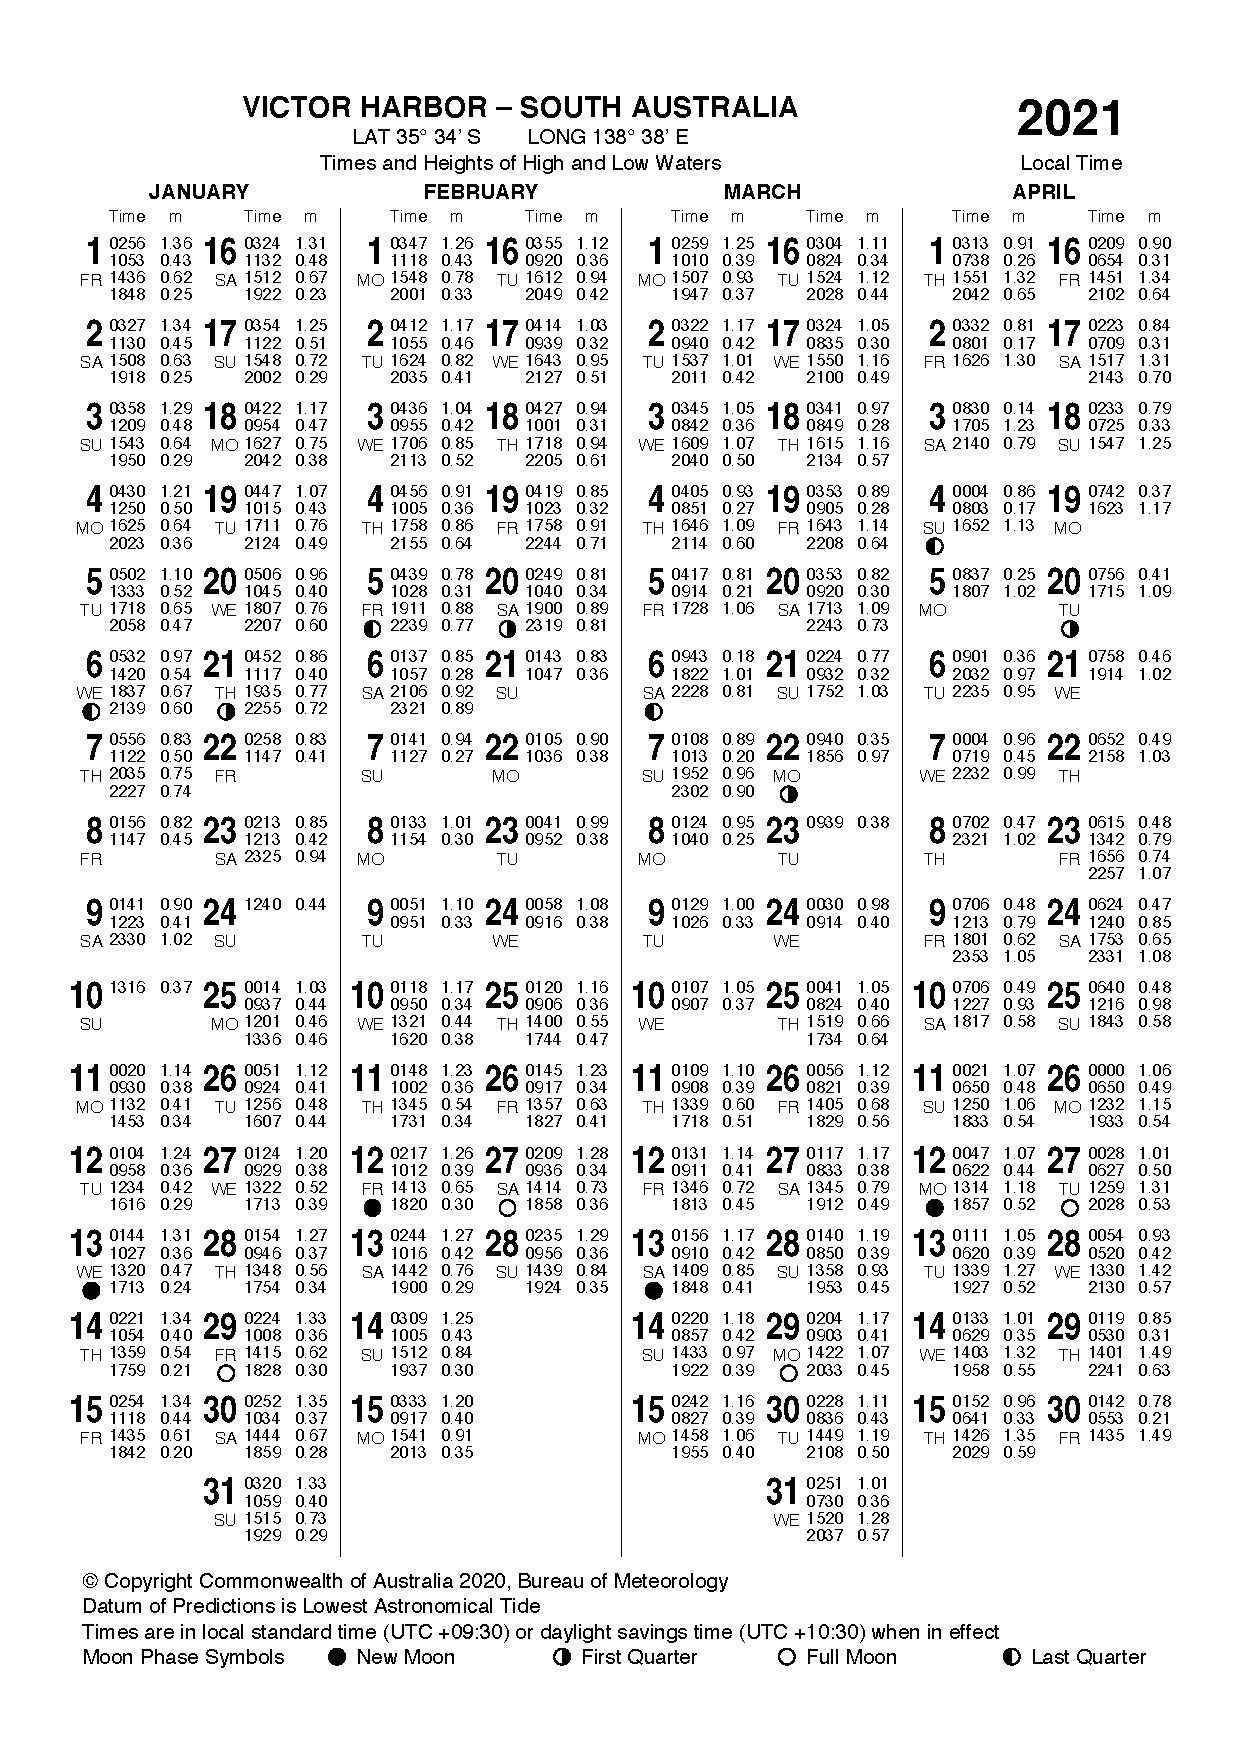
\includegraphics[height=0.4\textheight]{figures/images/IDO59001_2021_SA_TP006.pdf}
    \end{figure}
    forecast and filter?
    tsunami, 
\end{minipage}

\hfill

\begin{minipage}{0.45\textwidth}
    \begin{figure}      
     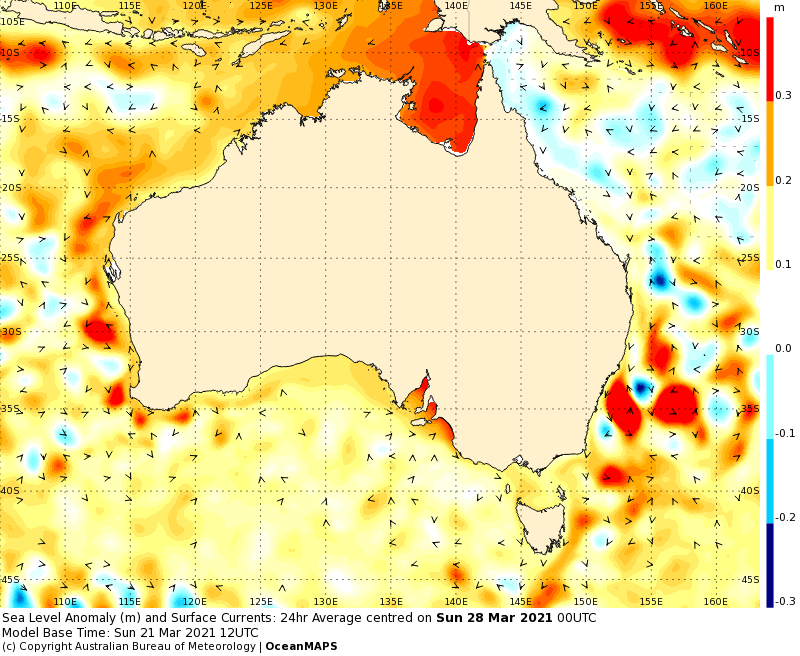
\includegraphics[width=\textwidth]{figures/images/IDYOC300.Aus.SLACur.168.png}
    \end{figure}
    altimeters - corrections
\end{minipage}


\end{frame}
%-----------------------------------------
\begin{frame}
\frametitle{Forecasts, physics, filters}

      \begin{figure}      
        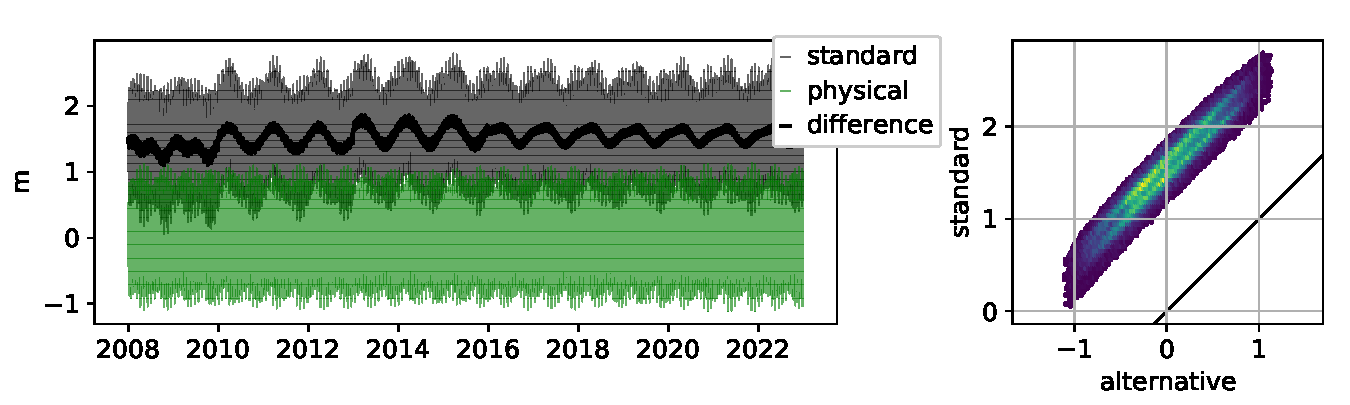
\includegraphics[width=\textwidth]{figures/plots/piecewiseTide_62430.pdf}
      \end{figure}

      \begin{itemize}
          \item standard annual tables - discontinuous
          \item contrast purpose and context
      \end{itemize}

\end{frame}
%-----------------------------------------
\begin{frame}
\frametitle{Global versus ``standard'' tides}
\begin{columns}
    \begin{column}{0.7\textwidth}
      \begin{figure}      
        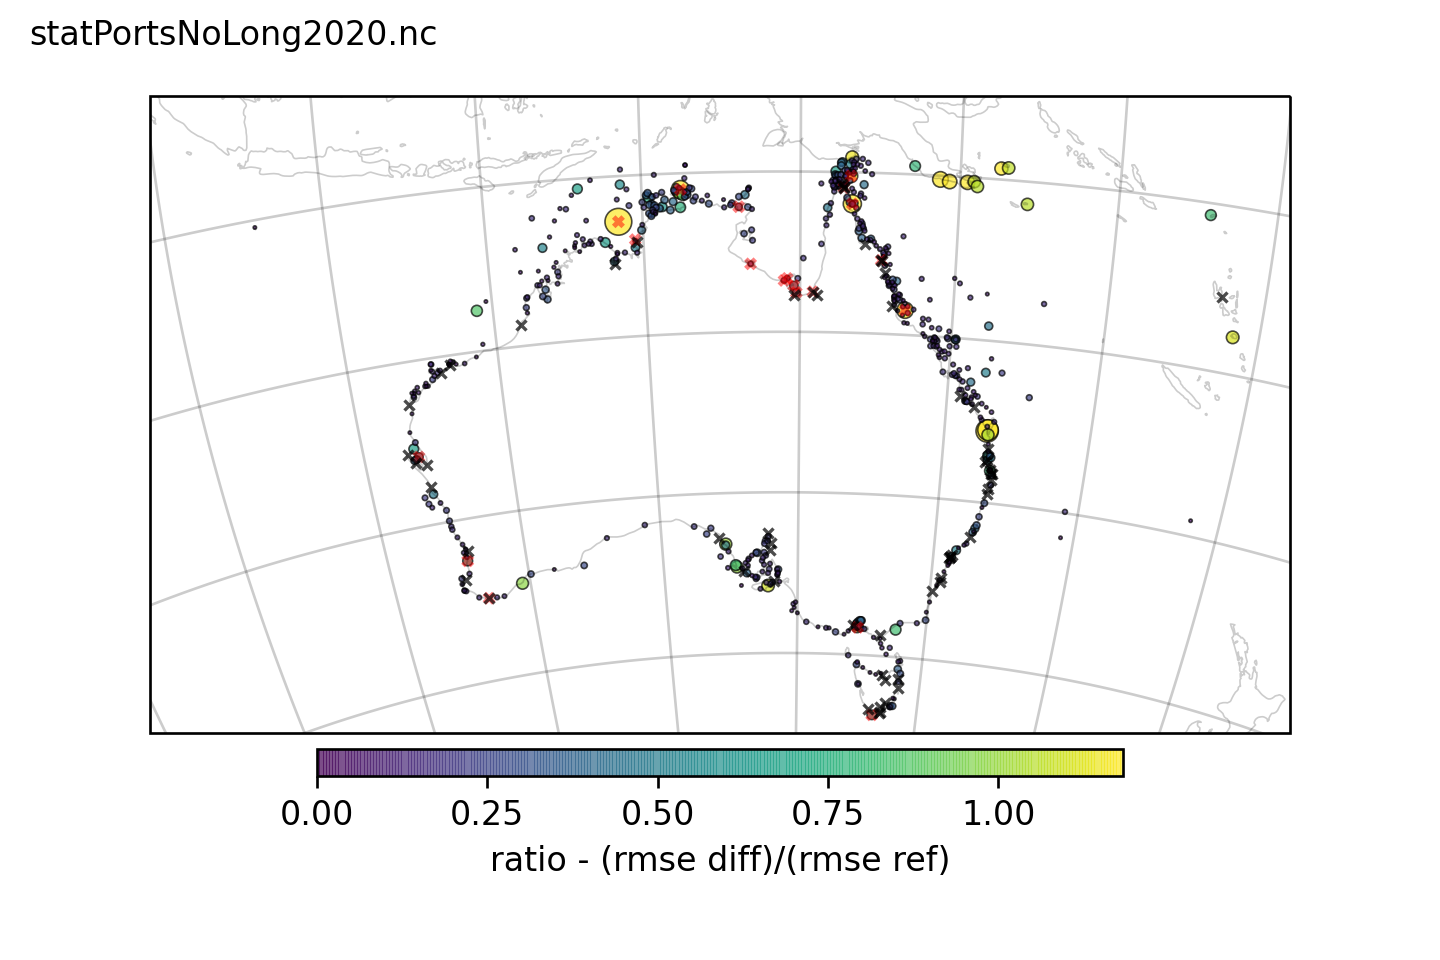
\includegraphics[width=\textwidth]{figures/maps/portsdiffRmseRatioNoLong.png}
      \end{figure}
    \end{column}

    \begin{column}{0.3\textwidth}
      \begin{figure}      
        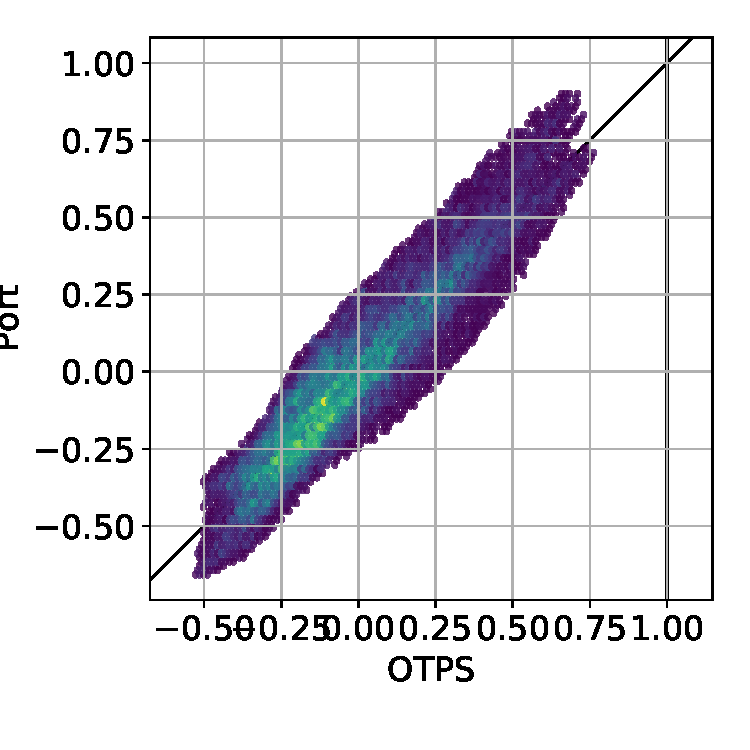
\includegraphics[height=0.25\textheight]{figures/plots/compareTides_61561_Full2020.pdf}
        \\
        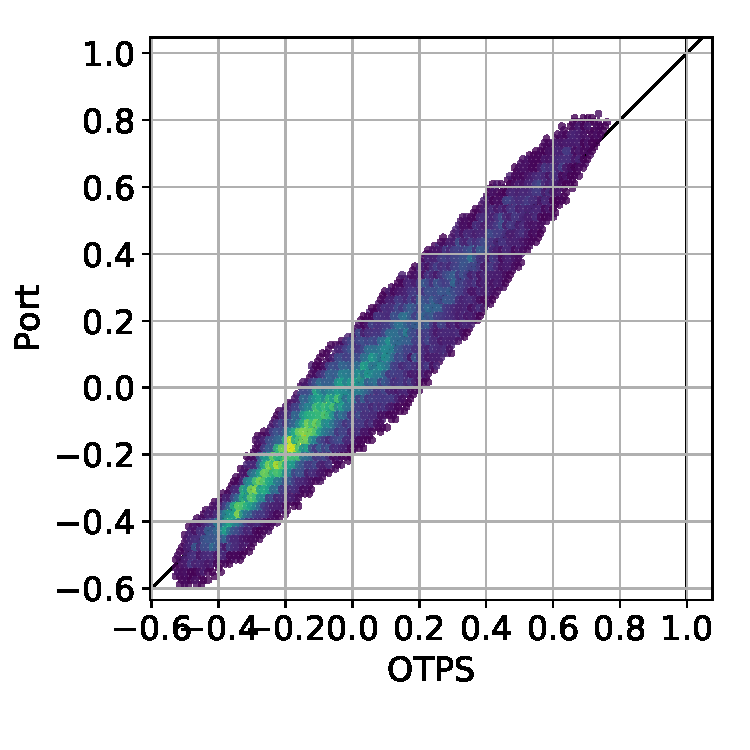
\includegraphics[height=0.25\textheight]{figures/plots/compareTides_61561_2020_201.pdf}
        \\
        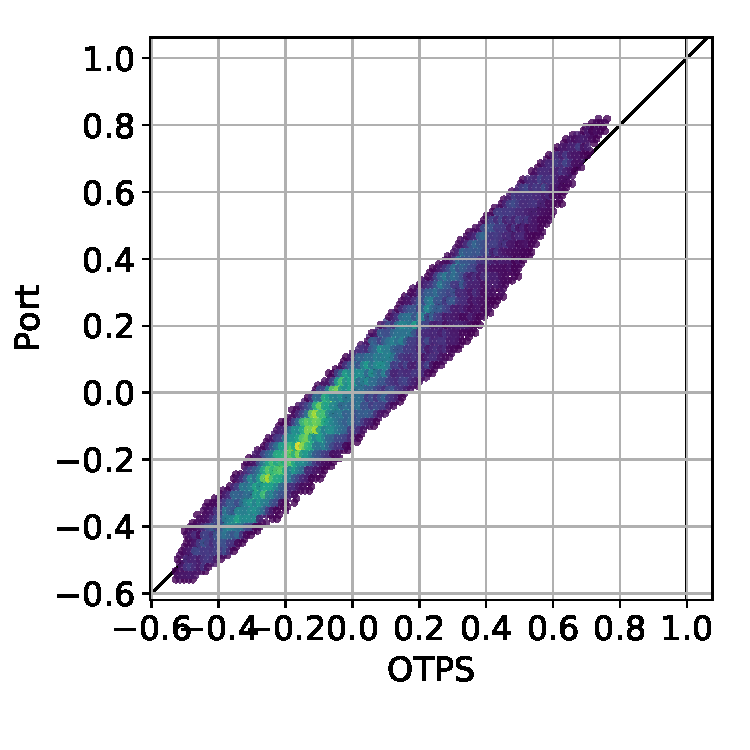
\includegraphics[height=0.25\textheight]{figures/plots/compareTides_61561_2020_105.pdf}
      \end{figure}
    \end{column}
\end{columns}
\end{frame}
%-----------------------------------------
\begin{frame}
\frametitle{Tidal service split}
      \begin{figure}      
        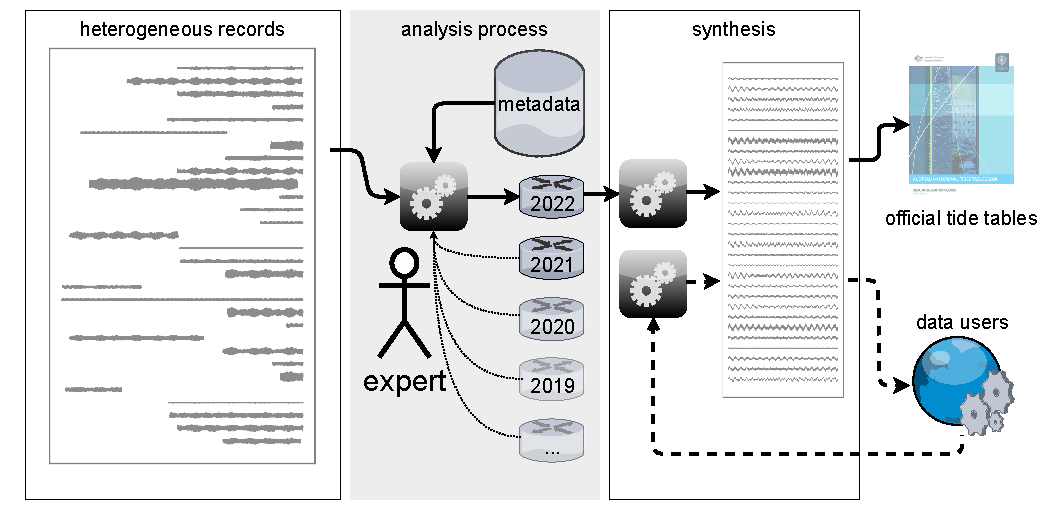
\includegraphics[height=0.6\textheight]{figures/diagrams/tideSchematic.pdf}
      \end{figure}
\end{frame}